\documentclass[12pt,a4paper,final,twoside,openright]{report}
\usepackage[utf8]{inputenc}
\usepackage[T1]{fontenc}
\usepackage[catalan]{babel}

\usepackage{setspace}
\onehalfspacing

\usepackage{graphicx}
\usepackage{caption}
\usepackage{amsmath}
\usepackage{hyperref}

\usepackage[left=2.5cm,right=2.5cm,top=2.5cm,bottom=2.5cm]{geometry}

\usepackage{fancyhdr}
\pagestyle{fancy}
\fancyhead{}
\fancyhead[RO,LE]{\thepage}
\fancyhead[RE,LO]{Control d'un doble integrador}
\fancyfoot{}
\fancyfoot[RO,LE]{
\includegraphics[scale=0.5]{Imatges/etseib.png}}


\usepackage{appendix}
\renewcommand{\appendixname}{Annexos}
\renewcommand{\appendixtocname}{Annexos}
\renewcommand{\appendixpagename}{Annexos}


\usepackage{chngcntr}
\counterwithin{figure}{chapter}%Permet que el comptatge de les figures sigui segons capitol
\counterwithin{table}{chapter}
\counterwithin{equation}{chapter}
\counterwithin{footnote}{chapter}

%PLANTEJAR TEMA DE \autoref{} ja que així l'hiperenllaç es també per la paraula i no sols el numero.

\renewcommand{\thefigure}{\arabic{chapter}.\arabic{figure}}
\renewcommand{\thetable}{\arabic{chapter}.\arabic{table}}
\renewcommand{\theequation}{\arabic{chapter}.\arabic{equation}}
\renewcommand{\thefootnote}{\arabic{footnote}}

\usepackage{etoolbox}
\patchcmd{\chapter}{\thispagestyle{plain}}{\thispagestyle{fancy}}{}{}

\headheight = 15pt %Donava un warning sino

\textheight = 690pt %Col·locació de l'escut a distancia que quedi be
\footskip = 60pt


\title{Tecnologia de Control \\ Control d'un doble integrador}
\author{Alumne: Lluís Salord Quetglas \\ Professor: Manel Velasco}
\date{Octubre 2015}

\begin{document}
%PENDENT QUE FUNCIONI L'INDEX
\maketitle
\thispagestyle{empty}

\cleardoublepage

\setcounter{page}{1} %Començar en la pagina 1

\begin{abstract}
\addcontentsline{toc}{chapter}{Resum}

Text de prova. Text de prova. Text de prova. Text de prova. Text de prova. Text de prova. Text de prova. Text de prova. Text de prova. Text de prova. Text de prova. Text de prova. Text de prova. Text de prova. Text de prova. Text de prova. Text de prova. Text de prova. Text de prova. Text de prova. Text de prova. Text de prova. Text de prova. Text de prova. Text de prova. Text de prova. Text de prova. Text de prova. Text de prova. Text de prova. Text de prova. Text de prova. Text de prova. Text de prova. Text de prova. Text de prova. Text de prova. Text de prova. Text de prova. Text de prova. Text de prova. Text de prova.

\end{abstract}

\tableofcontents

\listoffigures

\listoftables

\chapter{Introducció}

En l'àmbit d'aquesta assignatura es pretén aplicar els diferents coneixements de control de plantes que s'han adquirit al llarg de la carrera. Com a primera planta s'ha plantejat la d'un \textit{DI} (doble integrador). En aquest cas, pel fet de ser un doble integrador té dos pols en el zero i per tant és per ella mateixa una planta inestable.

En aquest informe es pretén explicar els procediments que s'han seguit per dur a terme el control d'aquesta planta amb els diferents mètodes utilitzats, argumentant quines implicacions té cadascun d'aquests. El control és du a terme a través d'una placa Arduino que es connecta directament a la placa a controlar.

Els diferents mètodes que s'han utilitzat per fer el control primer s'han simulat i fet els càlculs amb \texttt{Matlab} i la \textit{toolbox} \texttt{Simulink}. Tot seguit, s'ha connectat l'Arduino a l'ordinador per introduir-hi i executar el codi de control per finalment connectar la placa a controlar amb l'Arduino.



\section{Planta a controlar}

En aquest cas la planta a controlar és un placa que conté un doble integrador. El fet de tenir dos pols en el zero provoca que sigui inestable. L'esquemàtic del doble integrador és el que s'il·lustra a la figura \ref{fig:doble_int_scheme}.

 Aquesta placa té diverses connexions per tal de comunicar-se amb l'exterior i que sigui controlable de diverses formes. Aquestes són, per una banda, les entrades de 5 V i l'acció de control \textit{u}; i per altra banda, els punts $V_1$, $V_2$ i el \textit{GND} (0 V del circuit). La relació de les connexions entre el doble integrador i l'Arduino és la que es mostra en la taula \ref{tab:con_DI_Ard}. En aquestes connexions sobretot s'ha de tenir en compte que les entrades pel \textit{DI}, són sortides per l'Arduino i a l'inrevés. Per tant, \textit{D6} s'ha de configurar com a sortida, a més de tipus \textit{PWM}, i per altra banda, \textit{A5} i \textit{A6} com a entrades en l'Arduino.

\begin{figure}[h]
\centering
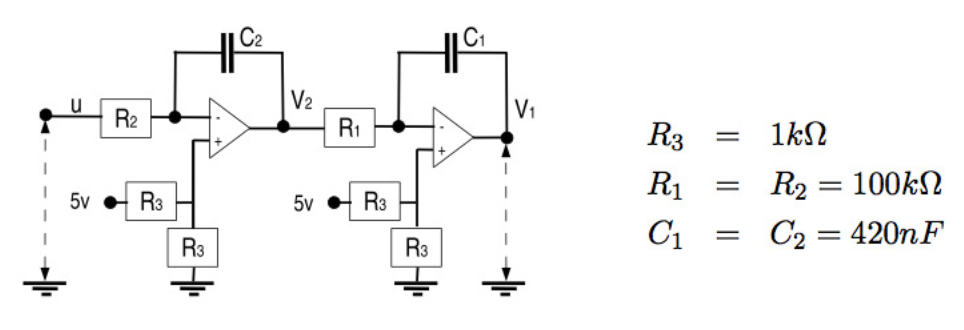
\includegraphics[width=0.8\textwidth]{Imatges/circuit_scheme.png}
\caption{Esquemàtic del doble integrador instal·lat a la placa \label{fig:doble_int_scheme}}
\end{figure}

\begin{table}[h]
\begin{center}
\begin{tabular}{l|l}
Arduino & Doble Integrador\\
\hline
5v & 5v (LM358N power)\\
IOREF & 5v (voltage divider input)\\
GND & GND\\
A5 & $V_1$ DI output voltage\\
A4 & $V_2$ DI output voltage\\
D6 & u (PWM)
\end{tabular}
\caption{Taula de connexions entre el doble integrador i ports de l'Arduino \label{tab:con_DI_Ard}}
\end{center}
\end{table}

\newpage %Per no tallar el paragraf amb les figures superiors
Finalment, sobre el \textit{DI} només queda comentar el model matemàtic d'aquest. Desenvolupant les equacions de la dinàmica del circuit electrònic de la figura \ref{fig:doble_int_scheme} s'arriba a les equacions \eqref{eq:V1} i \eqref{eq:V2}. A partir d'aquestes equacions i dels valors numèrics de la figura \ref{fig:doble_int_scheme} s'arriba al model matemàtic del doble integrador que s'utilitza, expressat com \eqref{eq:DI_model_1}, \eqref{eq:DI_model_2} i amb els valors de \eqref{eq:DI_values} per les matrius del sistema de la planta .

\begin{eqnarray}
\dot{V_1} = - \frac{u}{R_2 C_2}\label{eq:V1} \\
\dot{V_2} = - \frac{V_2}{R_1 C_1}\label{eq:V2}
\end{eqnarray}

\begin{equation}\label{eq:DI_model_1}
\begin{bmatrix}
\dot{x_1}\\
\dot{x_2}
\end{bmatrix}
=
A_g
\begin{bmatrix}
x_1\\
x_2
\end{bmatrix}
+
B_g
u
\end{equation}

\begin{equation}\label{eq:DI_model_2}
y = C_g
\begin{bmatrix}
x_1\\
x_2
\end{bmatrix}
+ D_g
\end{equation}

\begin{equation}\label{eq:DI_values}
A_g = \begin{bmatrix}
0 & -23.8095\\
0 & 0
\end{bmatrix}
~~
B_g = \begin{bmatrix}
0 \\
-23.8095
\end{bmatrix}
~~
C_g = \begin{bmatrix}
1 & 0
\end{bmatrix}
~~
D_g = 0
\end{equation}

\newpage
\section{Metodologia}

En aquesta assignatura es treballa directament amb la planta a controlar i l'Arduino que és la que porta el control d'aquesta. Ara bé, abans d'implementar el control primer s'han de fer les simulacions pertinents. A més, en haver-se incorporat el codi de control en l'Arduino, s'ha de comprovar que aquest s'està duent a terme de forma correcte. Aquesta metodologia de treball és du a terme en cadascun dels tipus de control que es duen a terme en el treball. Tot seguit s'explica en detall quines accions i programari s'utilitza per fer-ho.

El primer és dur a terme la simulació del conjunt planta-controlador. Aquesta es fa amb la \textit{toolbox} \texttt{Simulink} havent fet els càlculs previs amb \texttt{Matlab}, tals com matrius d'alguns sistemes o valors dels controlador. En les simulacions s'extreuen les dades que es creguin convenients per tal d'esser analitzades, tant per comprovar si el sistema es controlat teòricament amb precisió, com per esser contrastades després amb les dades reals.

En tenir el sistema simulat i amb un controlador adient s'ha de procedir a implementar aquest a través de l'Arduino. Per fer-ho s'han de transformar el conjunt de blocs de simulació a equacions i codi. Aquesta tasca és més complicada del que sembla, aquí es demostra com de clars es tenen els coneixements i és molt fàcil equivocar-se en algun punt, tot i ser un simple detall.

Finalment s'ha de comprovar el bon funcionament del control. Per dur a terme aquesta fase el primer és tenir alguna sortida de dades del sistema real. En aquest cas, s'utilitza el \texttt{Serial Port} de l'Arduino on a través de les funcions \texttt{Serial.print} i \texttt{Serial.println} esdevenen sortides del que es desitgi. Per l'estudi en qüestió s'envien les variables que intervenen en el sistema al \texttt{Serial Port} com són: les variables d'estat $V_1$ i $V_2$, la referència, l'acció de control $u$ i altres variables que poden ser importants segons el control que es faci. Al treure les dades pel \texttt{Serial Port}, si s'envien seguint cert patrons, poden ser llegides i plotejades \textit{online} amb el programa \texttt{KST} per exemple, o també poder ser emmagatzemades en un fitxer per després ser analitzades amb \texttt{Matlab}. Amb les dades plotejades es pot comprovar la precisió del control o comparar-les amb les dades extretes de les simulacions.

\chapter{Control de la planta}

La planta d'estudi es pot arribar a controlar de diverses formes, portant totes elles a l'estabilitat. Algunes porten l'estat a la referència amb més imprecisió que d'altres, com es comprova al llarg del treball, però totes elles provoquen que la planta sigui estable, que és l'objectiu del control. En aquesta part del treball és pretén explicar com s'han duit a terme els diferents controls i les característiques de cadascun d'ells.

\section{Control continu}

El control més senzill que es pot arribar a fer és considerar que el conjunt del sistema, planta-controlador, és en temps continu. En aquest cas, el sistema tan sols requereix del bloc de la planta, que utilitza els valors de les matrius de l'equació \eqref{eq:DI_values}, i una realimentació d'estat $K$, tal que els pols de llaç tancat siguin de part real negativa o nul·la (només si es un pol simple). Aquest tipus de sistema és simula amb l'esquemàtic de la figura \ref{fig:cont_scheme}.

\begin{figure}
\centering
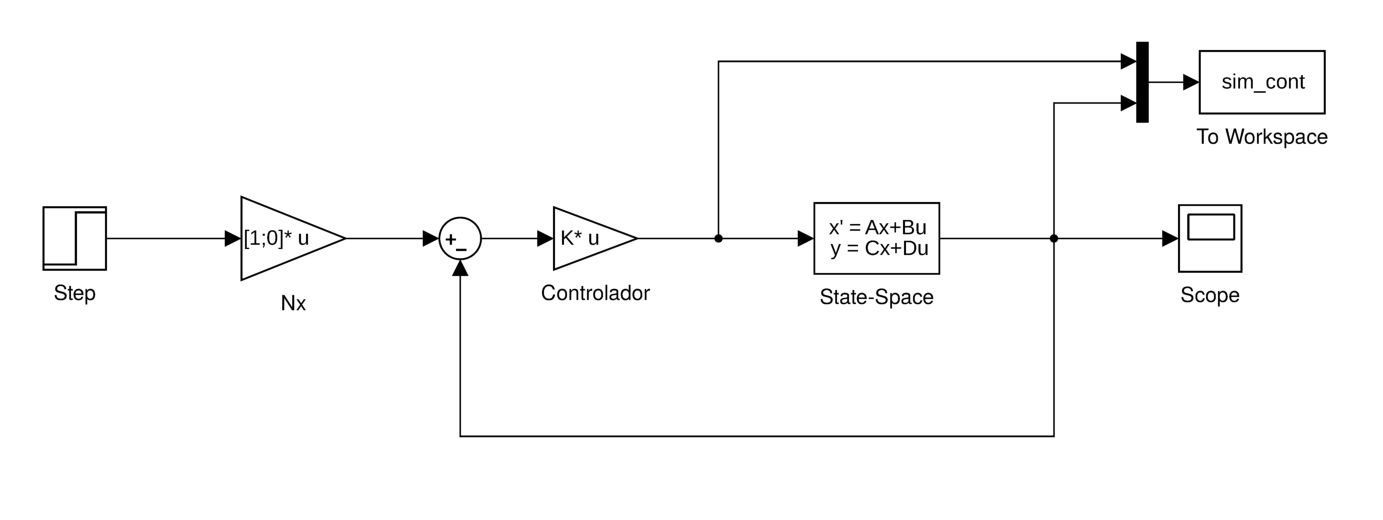
\includegraphics[width=0.8\textwidth]{Imatges/cont_sim_scheme.pdf}
\caption{Esquematic del sistema amb control continu\label{fig:cont_scheme}}
\end{figure}

A banda del que s'acaba d'explicar, en la figura \ref{fig:cont_scheme} també apareixen una referència que es pretén seguir i el bloc $N_x$. Aquest permet que el sistema segueixi la referència donada. Per altra banda, també s'hi hauria d'incloure un bloc $N_u$ que multiplicaria la referència i es sumaria a l'acció de control $u$ a l'entrada de la planta, però com es veu en els càlculs de les equacions \eqref{eq:Nx_Nu}, $N_u$ és igual a zero. El sistema \eqref{eq:Nx_Nu} surt de desenvolupar els requisits \eqref{eq:req_N} per tal que es segueixi la referència. 

\begin{equation}\label{eq:req_N}
\left\{
\begin{array}{lr}
N_x r = x_r = x_ss \\
C_r X_ss = y_r = r
\end{array}
\right.
\end{equation}

\begin{equation}\label{eq:Nx_Nu}
\begin{bmatrix}
N_x\\
N_u
\end{bmatrix}
=
\begin{bmatrix}
A_g & B_g\\
C_g & 0
\end{bmatrix}^{-1}
\begin{bmatrix}
0\\
0\\
1
\end{bmatrix}
=
\begin{bmatrix}
1\\
0\\
0
\end{bmatrix}
\Rightarrow \left\{
\begin{array}{lr}
N_x = \begin{bmatrix}
1\\
0
\end{bmatrix} \\
N_u = 0
\end{array}
\right.
\end{equation}

Un cop es té el sistema montat de tal manera que aquest pugui seguir una referència, s'ha de buscar el controlador $K$ tal que porti el sistema a error zero. Per aconseguir-ho, existeixen diverses formes depenent de si es pensen imposar uns pols de llaç tancat determinats (per assignació de pols o amb la formula d'Ackermann) o si es pretén fer un control òptim a partir d'una funció de cost determinada (control \texttt{LQR}). En el cas d'estudi, s'utilitza la formula d'Ackermann imposant un pols de llaç tancat amb part real negativa o nul·la (només si és un pol simple).

Els pols que s'han d'imposar com s'ha dit abans han de ser uns que siguin de part real negativa o nul·la. Ara bé, en aquest sistema s'han d'escollir dos pols, per tant, aquests no poden ser de part real nul·la ja que farien el sistema inestable. Finalment, s'han escollit els pols $-5\pm20i$ que compleixen el requisit i que ha sigut proposat pel professor. 

Un cop escollits els pols tan sols queda aplicar la formula d'Ackermann. Aquesta dona el valor $K$ del controlador donats els pols desitjats i les matrius $A$ i $B$ del sistema. Al cap i a la fi, dona el mateix resultat que l'assignació de pols on s'iguala el polinomi característic desitjat amb $|z \mathbf{I} - (\mathbf{A_g} - \mathbf{B_g K})|$. La formula consisteix en l'equació \eqref{eq:Acker} on $p_d(A_g)$ és el polinomi característic desitjat amb el valor de la matriu $A_g$. En el \texttt{Matlab} la funció \texttt{acker} s'encarrega de fer aquests càlculs. Si es desitja llegir el codi \texttt{Matlab} utilitzat per fer tots els càlculs es pot trobar en l'Annex \ref{ann:mat_cont}.

\begin{equation}\label{eq:Acker}
K=(0\quad0\quad0\quad\dots\quad1)(\mathbf{A_g}\quad \mathbf{A_g B_g}\quad \mathbf{A_g^2 B_g}\quad \dots\quad \mathbf{A_g^{n-1} B_g})^{-1} p_d(A_g)
\end{equation}

Al tenir tots els valors es procedeix a dur a terme les simulacions. Les dades plotejades es mostren en la figura \ref{fig:cont_sim}. Aquí es pot veure com, en la simulació, s'aconsegueix estabilitzar la planta, tot i venir d'unes condicions inicials diferents a zero. Ara bé, aquesta simulació no s'adapta a la realitat, ja que l'Arduino envia l'acció de control de forma discreta i per tant el control no es correcte. Tot i que en aquest cas s'ha comprovat experimentalment que igualment es controla, tot i que no de la forma desitjada. Per tant, d'aquest tipus de control no se'n fa l'anàlisi experimental amb l'Arduino. 

\begin{figure}
\centering
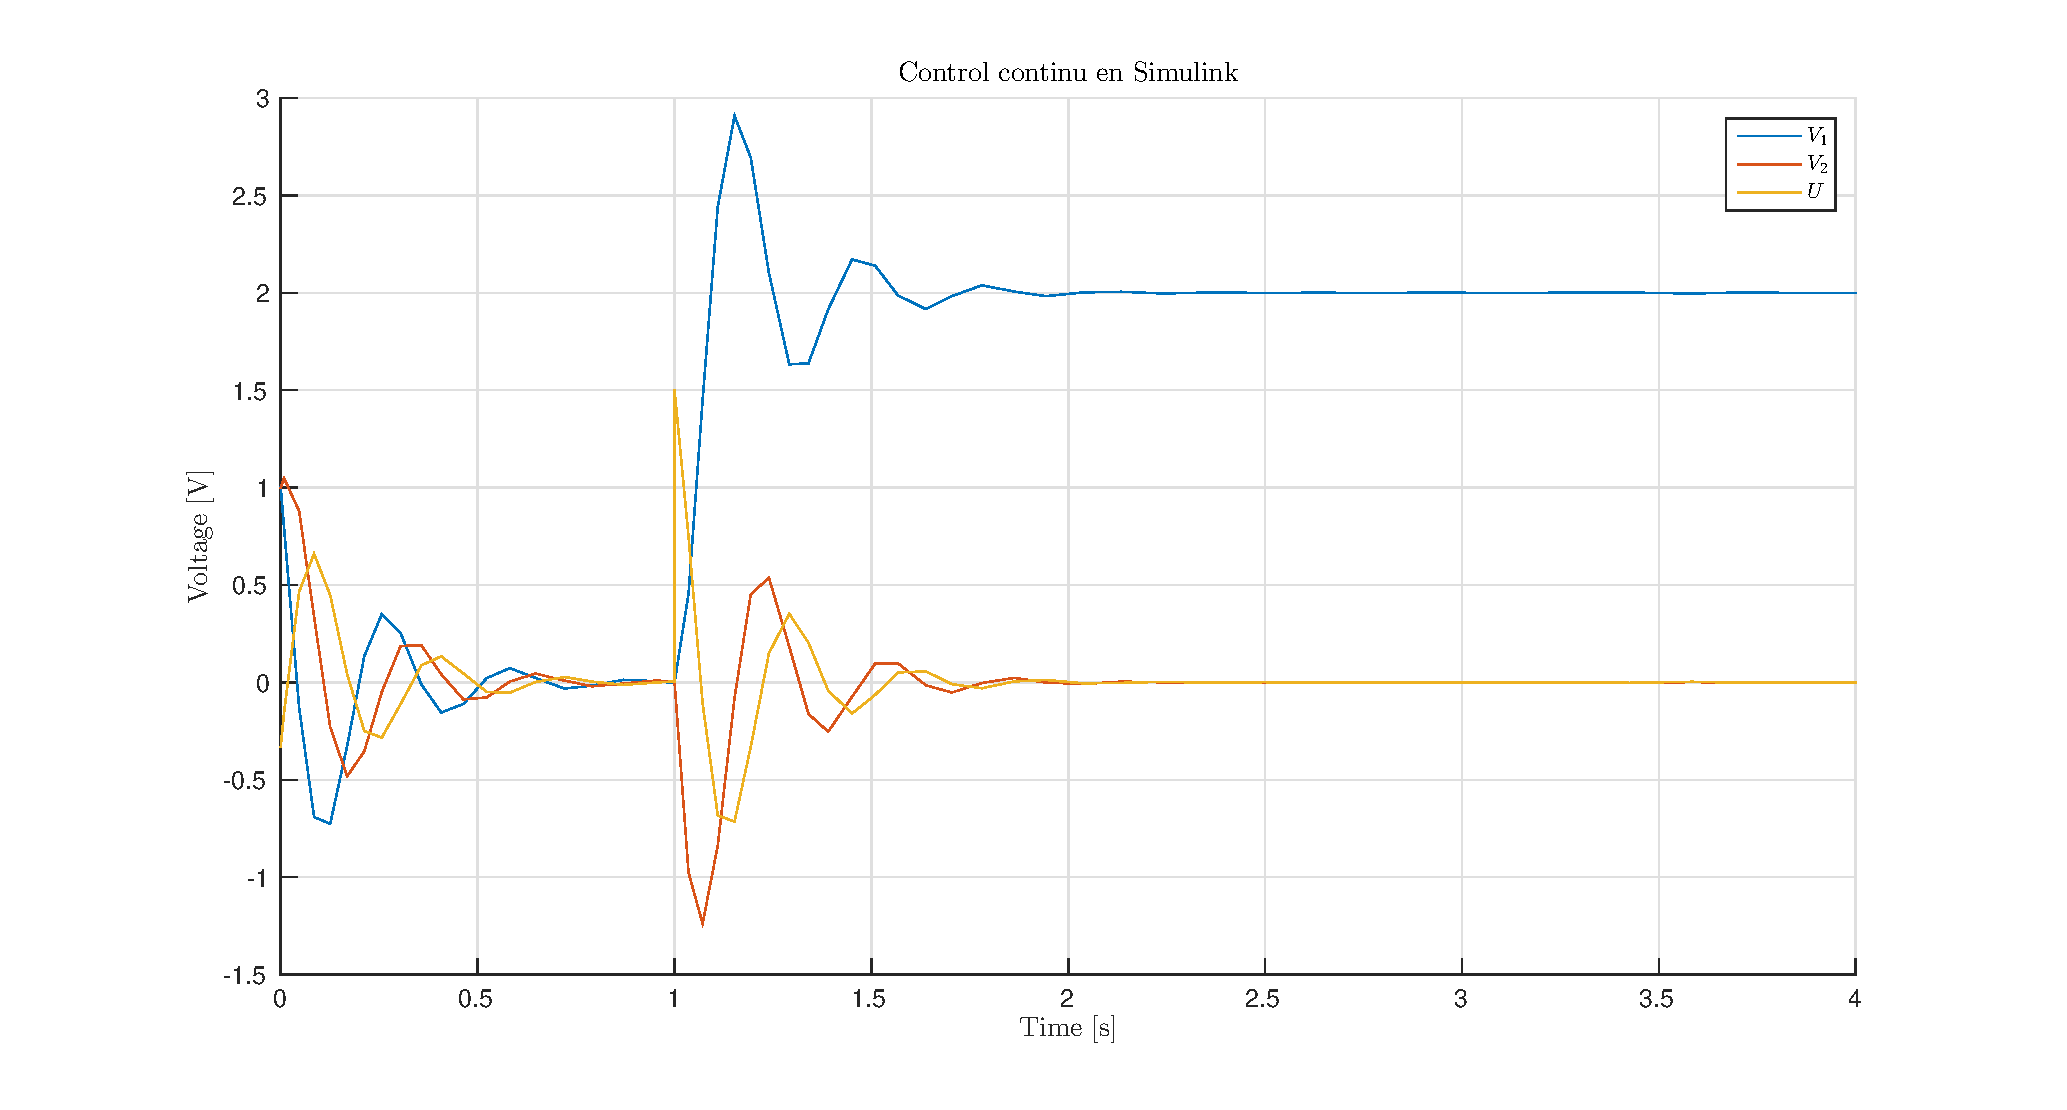
\includegraphics[width=0.8\textwidth]{Imatges/cont_sim.eps}
\caption{Dades de la simulació amb control continu\label{fig:cont_sim}}
\end{figure}

D'aquest cas no se'n fa un anàlisi en profunditat ja que no té especialment sentit físic. Només destacar, com es veu en la figura \ref{fig:cont_sim}, el fet que es demostra que una planta inestable, amb el controlador adequat por permetre l'estabilització del sistema.

\section{Control discret}

Com s'ha explicat en el cas del control continu, aquest no reflecteix la realitat, ja que el controlador (l'Arduino) funciona de forma discreta. Aquest llegeix les dades i fa els càlculs un cop cada cert temps, i envia el mateix valor del senyal durant aquest període.

El fet que es consideri el controlador discret no s'ha de confondre en que la planta funcioni de forma discreta. La planta és continua, l'únic que passa és que l'entrada, almenys la part que prové del controlador, és discreta i per tant el controlador s'ha d'adaptar a aquest tipus de funcionament. 

El primer que s'ha de fer és saber a quina freqüència treballa el controlador. En aquest cas, s'ha estipulat en l'enunciat un funcionament a $20 Hz$ (període de mostreig de $0.05 s$). Posteriorment, s'han de plantejar els pols de llaç tancat del sistema. Per simplificar, s'han escollit els mateixos que en el control continu, però discretitzats, que és fa aplicant l'equació \eqref{eq:pol_dis} als pols continus, sent $T_s$ el període de mostreig del controlador. Aplicant \eqref{eq:pol_dis} als pols continus, $-5\pm20i$, de l'apartat anterior, en resulten els pols discrets $0.4208\pm0.6553i$. El mòdul d'aquests pols és $0.7788$ es troben dins el cercle unitari, per tant, són estables. 

\begin{equation}\label{eq:pol_dis}
P_{dis} = e^{T_s P_{cont}}
\end{equation}


Per últim càlcul queda la $K$ del controlador, que es designa al llarg de treball com $K_{dis}$. Per tal d'aconseguir-ho també es pretén utilitzar la formula d'Ackermann \eqref{eq:Acker}, però no s'utilitzen les matrius $A_g$ i $B_g$, sinó les seves transformacions al sistema discret amb el període de mostreig $T_s$. Això es pot fer a través de la funció \texttt{c2d} del \texttt{Matlab}, on donades les matrius del sistema continu i el període de mostreig $T_s$ dona les matrius $\Phi$ i $\Gamma$ del sistema discret. Finalment, s'introdueixen les matrius $\Phi$ i $\Gamma$ i el període de mostreig a la funció \texttt{acker} i es té com a resultat el controlador $K_{dis}$.

\section{Control amb observador}

\section{Control amb refús de pertorbació}

\subsection{Pertorbació constant}

\subsection{Pertorbació sinusoïdal}

\subsection{Pertorbació constant i sinusoïdal}

\section{Ús de pols reals de l'observador}
%S'ha vist que hi ha unes freqüencies molt altes i s'ha pensat en que poden ser degudes als pols de l'observador que s'han posat, per això es decideix a procedir amb l'ús de pols reals en lloc dels proposats a l'inici.
%Després també es veu com el fet que siguin ràpids no es necessari ja que es preten refusar un senyal que es sempre igual. Es veu en la transformada de fourier.

%\bibliography{./Bibliografia/library}
%\addcontentsline{toc}{chapter}{Referències}
%\label{Referencies}


\appendix
\clearpage % o \cleardoublepage
\addappheadtotoc
\appendixpage

\chapter{Matlab}

\section{Control continu}\label{ann:mat_cont}
\begin{verbatim}
%parametres model
A= [0 -23.8095;0 0];
B= [0;-23.8095];
C= [1 0];
D=[0;0];

%buscar controlador continu(realimentacio)
P=[-5+20i,-5-20i];
K=acker(A,B,P);

%busco parametres Nu i Nx
W=[A B;C 0];
N=inv(W)*[0;0;1];
Nx=N(1:2);
Nu=N(3);
\end{verbatim}

\section{Control discret}\label{ann:mat_dis}

\begin{verbatim}
%parametres model
A= [0 -23.8095;0 0];
B= [0;-23.8095];
C= [1 0];
D=[0;0];


%pols de llaç tancat en continu
P=[-5+20i,-5-20i];

%buscar controlador discret
h=5E-2;
[phi, gam] = c2d(A,B,h);
P_dis=[exp(P(1)*h), exp(P(2)*h)];
K_dis=acker(phi,gam,P_dis);

%busco parametres Nu i Nx
W=[phi-eye(2) gam;C 0];
N=inv(W)*[0;0;1];
Nx=N(1:2);
Nu=N(3);
\end{verbatim}

\section{Control amb observador}\label{ann:mat_obs}
\begin{verbatim}
%parametres model
A= [0 -23.8095;0 0];
B= [0;-23.8095];
C= [1 0];
D=[0;0];

%pols de llaç tancat en continu
P=[-5+20i,-5-20i];

%buscar controlador discret
h=5E-2;
[phi, gam] = c2d(A,B,h);
P_dis=[exp(P(1)*h), exp(P(2)*h)];
K_dis=acker(phi,gam,P_dis);

%busco parametres Nu i Nx
W=[phi-eye(2) gam;C 0];
N=inv(W)*[0;0;1];
Nx=N(1:2);
Nu=N(3);

%buscar controlador de l'observador amb pols més ràpids que la planta
P_obs=[-10+20i,-10-20i];
P_obs_dis=exp(P_obs.*h);
K_obs_dis=acker(phi', C', P_obs_dis);
L=K_obs_dis';
C_obs=eye(2);
\end{verbatim}

\section{Control amb refús de pertorbació}\label{ann:mat_pert}

\subsection{Pertorbació constant}\label{ann:mat_pert_ct}
\begin{verbatim}
%Control amb refus de perturbacions (Cas perturbacions constants)
%parametres model
A= [0 -23.8095;0 0];
B= [0;-23.8095];
C= eye(2);
D=[0;0];

%buscar controlador continu(realimentacio)
P=[-5+20i,-5-20i];
h=5E-2;
[phi, gam] = c2d(A,B,h);
P_dis=[exp(P(1)*h), exp(P(2)*h)];
K_dis=acker(phi,gam,P_dis);


phi_pert=[phi gam; 0 0 1];
gam_pert=[gam; 0];
C_pert=eye(3);

P_obs=[-10+20i,-10-20i];
P_obs_dis_pert=[exp(P_obs.*h), 0.9];
K_obs_dis_pert=acker(phi_pert', [1 0 0]', P_obs_dis_pert);
L_pert=K_obs_dis_pert';
\end{verbatim}

\subsection{Pertorbació sinusoïdal}\label{ann:mat_pert_sin}
\begin{verbatim}
%Control amb refus de perturbacions (Cas perturbacions sinusoidals)
%parametres model
A= [0 -23.8095;0 0];
B= [0;-23.8095];
C= eye(2);
D=[0;0];
%buscar controlador discret
P=[-5+20i,-5-20i];
h=5E-2;
[phi, gam] = c2d(A,B,h);
P_dis=[exp(P(1)*h), exp(P(2)*h)];
K_dis=acker(phi,gam,P_dis);

w=2.4*2*pi();
phi_sin=c2d([0 1;-w*w 0],[1 0]',h);
phi_pert=[phi gam [0;0]; zeros(2) phi_sin];
gam_pert=[gam; 0; 0];
C_pert=eye(4);

P_obs=[-10+20i,-10-20i];
P_obs_dis_pert=[exp(P_obs.*h), 0.3, 0.3];
K_obs_dis_pert=acker(phi_pert', [1 0 0 0]', P_obs_dis_pert);
L_pert=K_obs_dis_pert';
\end{verbatim}


\subsection{Pertorbació constant i sinusoïdal}\label{ann:mat_pert_ct_sin}
\begin{verbatim}
%Control amb refus de perturbacions (Cas perturbacions sinusoidals i constants)
%parametres model
A= [0 -23.8095;0 0];
B= [0;-23.8095];
C= eye(2);
D=[0;0];

%buscar controlador discret
P=[-5+20i,-5-20i];
h=5E-2;
[phi, gam] = c2d(A,B,h);
P_dis=[exp(P(1)*h), exp(P(2)*h)];
K_dis=acker(phi,gam,P_dis);

w=2.4*2*pi();
phi_sin=c2d([0 1;-w*w 0],[1 0]',h);
phi_pert=[phi gam gam [0;0]; zeros(3,2) [1;0;0] [[0 0]; phi_sin]];
gam_pert=[gam; 0; 0; 0];
C_pert=eye(5);

P_obs=[-10+20i,-10-20i];
P_obs_dis_pert=[exp(P_obs.*h), 0.4, 0.4, 0.9];
K_obs_dis_pert=acker(phi_pert', [1 0 0 0 0]', P_obs_dis_pert);
L_pert=K_obs_dis_pert';
\end{verbatim}

\section{Ús de pols reals de l'observador}
\begin{verbatim}
%Control amb refus de perturbacions (Cas perturbacions sinusoidals i constants)
%parametres model
A= [0 -23.8095;0 0];
B= [0;-23.8095];
C= eye(2);
D=[0;0];

%buscar controlador discret
P=[-5+20i,-5-20i];
h=5E-2;
[phi, gam] = c2d(A,B,h);
P_dis=[exp(P(1)*h), exp(P(2)*h)];
K_dis=acker(phi,gam,P_dis);

w=0.5371*2*pi();
phi_sin=c2d([0 1;-w*w 0],[1 0]',h);
phi_pert=[phi gam gam [0;0]; zeros(3,2) [1;0;0] [[0 0]; phi_sin]];
gam_pert=[gam; 0; 0; 0];
C_pert=eye(5);

P_obs=[-10,-5];
P_obs_dis_pert=[exp(P_obs.*h), 0.9, 0.9, 0.9];
K_obs_dis_pert=acker(phi_pert', [1 0 0 0 0]', P_obs_dis_pert);
L_pert=K_obs_dis_pert';
\end{verbatim}

\section{Funció per plotejar amb format \LaTeX}\label{ann:mat_plot}
\begin{verbatim}
function plot_control(X,Y,title_plot,names, x_min, x_max, y_min, y_max)

set(0,'DefaultTextInterpreter', 'latex')

fontsize = 12;
set(0,'defaultaxesfontsize',fontsize);
set(0,'defaulttextfontsize',fontsize);

figure
hold on;

for i=1:length(Y(1,:))
plot(X,Y(:,i),'DisplayName',names(i));
end

title(title_plot);
xlabel('Time [s]', 'Interpreter', 'latex');
ylabel('Voltage [V]','Interpreter','latex');

axis([x_min x_max y_min y_max]);

h=legend(names);
set(h,'Interpreter', 'latex');

grid on;

end

\end{verbatim}

\chapter{Arduino}

\section{Control continu}

\section{Control discret}

\section{Control amb observador}

\section{Control amb refús de pertorbació}

\subsection{Pertorbació constant}

\subsection{Pertorbació sinusoïdal}

\subsection{Pertorbació constant i sinusoïdal}

\end{document}
